\chapter{Projekt}
\section{Architektura}
Architektura rozwiązania. Aplikacja stworzona będzie w architekturze klient-serwer. Interfejs użytkownika zrealizowany będzie w technolgii aplikacji internetowych, tak by dostęp do repozytorium nie wymagał instalacji i był dostępny na wszystie platformy. Dodatkowo stworzona zostanie usługa internetowa ( ang. web service ), tak by umożliwić zintegorowanie aplikacji z zewnętrznymi aplikacjami dzięki czemu możliwa będzie automatyzacja kluczowych procesów. Perzystencja danych dokonywana będzie w relacyjnej bazie danych poprzez moduł odwzorowujący obiektową architekturę systemu informatycznego na bazę danych.

Aplikacja zostanie napisana w języku JAVA. Język ten jest obecnie najczęśniej spotykanym językiem w zagadnieniach korporacyjnych. Posiada rozwinięte wsparcie społeczności i rozbudowane funkcjonalności wbudowane, jak i rozwijane przez zewnętrznych kontrybutorów. 
\begin{figure}[h]
\centerline{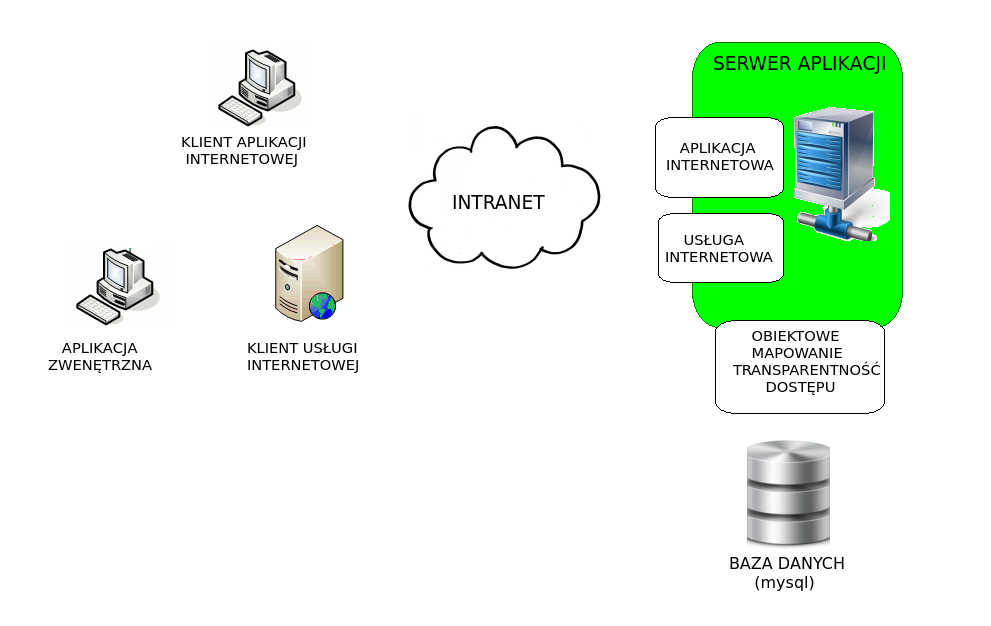
\includegraphics[scale=0.5]{img/architektura.png}}
\caption{Architektura systemu}
\label{fig:architektura}
\end{figure}


%<< Diagram fizyczny >>

%<< Diagram komponentów >>

%Komponent zarządzanie użytkownikami

%Komponent Definicji 

%Komponent wykonania testów

%Komponent danych dodatkwych
\section{Warstwy}
\subsection{Warstwa aplikacji internetowej}
Dostęp poprzez aplikację internetową jest podstawowym źródłem interakcji użytkowika w projektowanej aplikacji. Celem rozdzielenia poszczególnych odpowiedzialności modułów oprogramowania, użyty zostanie zworzec Model-Widok-Kontroler. Zakłada on wydzielenie trzech wartst:
\begin{enumerate}
  \item Model - odpowiedzialny za pobranie i enkapsulacje danych
  \item Widok - odpowiedzialny za wyświetlenie sformatowanej treści. Język stosowany w widoku powinien pozwalać na swobodne osadzanie treści języka końcowego ( w tym przypadku HTML ), powinien on być dostosowany do edycji przez osoby nie posiadające wiedzy na temat języku programowania.
  \item Kontroller - odpowiedzialny za skoordynowanie pobrania danych, przetworzenia ich za pomocą serwisów i przesłanie danych do widoku
\end{enumerate}

Język JAVA oferuje kilka ustandaryzowanych technologii które pozwalają tworzyć aplikacje internetowe z wykorzystaniem wzorca Model-Widok-Kontroler. Zaprezentowana aplikacja stworzona zostanie w oparciu o technologię Java Server Faces i jej implementacje PrimeFaces.

Java Server Faces jest jednym ze standardów tworzenia aplikacji internetowych w języku JAVA\cite{jsfRef}. Główne założenia standardu to:
\begin{enumerate}
  \item Łatwość tworzenia części klienckiej ( widoku ) w oparciu o strukturę komponentową. Udostępnione są standardowe komponenty ( takie jak na przykład formularz, pole tekstowe ).
  \item Możliwość zagnieżdżania struktury dokumentu, pozwalająca na minimalizację redundancji po stronie szablonu strony internetowej 
  \item Ustandaryzowany dostęp z widoku do danych po stronie serweru
  \item Zapewnienie trwałości stanu danych pomiędzy żądaniami w obrębie sesji klienta
  \item Część serwerowa oparta jest na ziarnach ( JavaBeans ), posiada wsparcie dla walidacji zarówno po stronie klienckiej jak i serwerowej
\end{enumerate}

W technologii Java Server Faces rola Kontrolera rozdzielona jest na pliki szablonu strony i ziarna zarządzające po stronie serweru. W plikach szablonu osadzone są instrukcję które wprost pobierają danę z kontrolera i wykonują na nim akcje.

Standard Java Server Faces posiada wiele implementacji. W tworzonej aplikacji użyta została implementacja PrimeFaces\cite{primeFaces}. PrimeFaces jest rozwijany jako otwarty projekt. Implementacja ta rozszerza standard o własne komponenty, uproszcza również sposób komunikacji klient serwer poprzez AJAX ( asynchroniczna komunikacja poprzez język JavaScript)

\subsection{Warstwa usługi internetowej}

Przedsiębiorstwa informatyzują wiele kluczowych procesów biznesowych. Zdarza się iż do rozwiązania konkretnego przypadku stosowane jest kilka różnych systemów, pochodzących od jednego wydawcy lub wydawaców ze sobą niezwiąnych. Fakt istnienia różnych systemów powoduje konieczność zintegrowania ich wspólnie tak by systemy mogły w sposób zautomatyzowany wymieniać między sobą dane, zdarzenia, komunikaty.

Różnorodność na rynku informatycznym powoduje iż programy pracujące w tej samej domenie, używane wspólnie do rozwiązania konkretnej potrzeby biznesowej, tworzone są w różnych technologiach, w odmiennych językach programowania. Potrzeba komunikacji pomiędzy programami, które różnią się implementacją i technologiami rozwiązywana jest poprzez zastosowanie standardów które mogą być stosowane interdyscyplinarnie.

Jedym ze standardów komunikacji między aplikacjami jest komunikacja poprzez usługę internetową. 

Dodatkową warstwą dostępu jest dostęp poprzez technologię Web Service REST. Z tego poziomu dostępna jest tylko część funkcjonalnośći. Głównym zastosowaniem dostępu poprzez Web Service jest możliwość zintegrowania aplikacji z zewnętrznymi usługami.



Usługa internetowa pozwala na wykonanie trzech akcji:
\begin{enumerate}
  \item dodania wymagań, tak by w ten sposób móc zautomatyzować ten proces, na przykład dodając wprost z zewnętrzej bazy dedykowanej do przechowywania i śledzenia wymagań
  \item pobrania wykonania przypadków testowych dla użytkownika
  \item aktualizacji wykonania przypadku testowego. Udostępnienie dwóch powyższych podpunków pozwala na stworzenie osobnego modułu klienckiego
\end{enumerate}.

\subsection{Moduły aplikacji}
Funkcjonalności realizowane przez aplikację możemy podzielić na logicznę moduły.
\begin{figure}[h]
\centerline{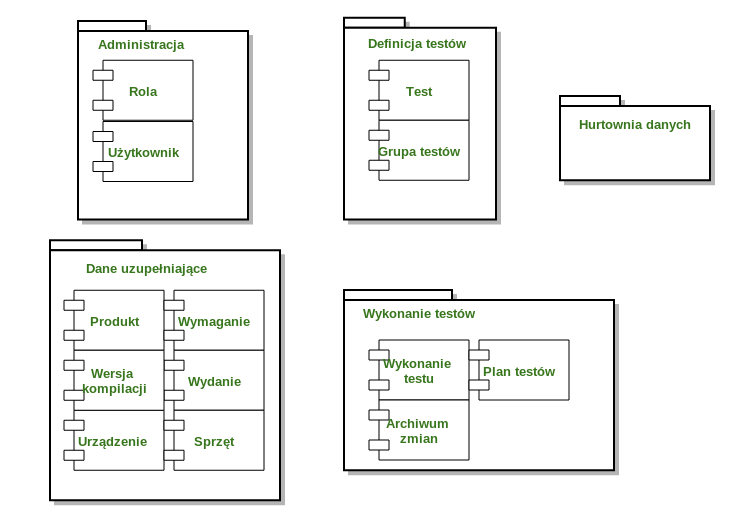
\includegraphics[scale=0.5]{img/komponenty.png}}
\caption{Mouły systemu}
\label{fig:moduly}
\end{figure}

\subsubsection{Moduł administracji}

Moduł ten skupia wszelkie funkcjonalności związane z zarządzaniem użytkownikami w systemie. Odpowida za tworzenie i edycję użytkowników. Każdy użytkownik posiada takie dane jak login, adres e-mailowy, hasło jak również przypisaną rolę.

Możemy wyróżnić kilka ról użytkowników. Rola określa jakie uprawnienia otrzymuje zalogowany użytkownik i określa widok ekranu początkowego. Każda z ról posiada charakterystyczne cechy które pokrywają role użytkowników w procesie testowania oprogramowania: menedżer testów, lider testów, inżynier testów, specjalista środowiska do testów, specjalista konfiguracji testowej \cite{peopleWare}. Poniżej zaprezentowany zostanie opis poszczególnych ról.
\begin{enumerate}
  \item Administrator --  zarządza użytkowikami w systemie. Administrator tworzy użytkowników i nadaje im uprawnienia.
  \item Koordynator testów -- tworzy przypadki testowe, grupy testów i scenariusze. Rola ta odpowiedzialna jest za treści merytoryczne repozytorium. Użytkownik odpowiada za utrzymanie testów, aktualizację ich, pokrycie funkcjonalności. 
  \item Obsługa techniczna -- rola ta odpowiedzialna jest za zapewnienie odpowiedniego środowiska dla testerów, konserwacje i naprawę fizycznych defektów. Użytkownik ten przypisany jest do konkretnych wykonań scenariuszy, instaluje początkowe środowisko, wymagane wersje oprogramowania, naprawia usterki sprzętowe.
  \item Lider testów -- wspiera zespół w wykonynwaniu scenariusza testowego. Służy swoją wiedzą i doświadczeniem przy podziale prac i podczas pojawiających się problemów. Posiada władzę decyzyjną przy zakwalifikowaniu testu jako nie udanego. Lider przypisuje testerów do testów.
  \item Tester --  wykonuje przypisane do niego przypadki testowe. Tester wykonuje przypadki testowe przypisane do niego. Oznacza stan testów i zgłasza napotkane problemy.
  \item Pośrednik ( ang. liason ) --  Odpowiedzialny jest za komunikacje zespołu testów z zespołem programistycznym. Posiaga wgląd do aktulnie wykonywanyh testów i konfiguracji. Jego zadaniem jest rozwiązywanie problemów związanych z jego macierzystym produktem. Pomaga zakwalifikować problem powstały podczas testów, szczególnie na początku testów produktu, zespół testerki może nie posiadać wystarczającej wiedzy i błędnie kwalifikować obserwowane rezultaty jako błąd produktu. Pośrednik proponuje również tymczasowe rozwiązania które pozwalają obejść problemy wynikające z błędów w oprogramowaniu, które naprawione będą dopiero podczas przyszłych wersji oprogramowania, tak by proces testowania mógł przebiegać nieprzerwanie.

  
\subsubsection{Moduł definicji}

\subsubsection{Moduł danych uzupełniających}

\subsubsection{Moduł wykonania }

\subsubsection{Moduł archiwum zmian }





\section{Składowe aplikacji}


Podstawową jednostą aplikacji jest przypadek testowy. Składa się on z :
\begin{enumerate}
  \item wymagana konfiguracja, warunków wejściowych
  \item scenariusz, to jest lista kroków do wykonania wraz z oczekiwanymi rezultatami
  \item wymagania które są weryfikowane 
  \item opis
  \item tytuł
  \item identyfikator
  \item estymowany czas potrzebny do wykonaniu
  \item lista urządzeń wymaganych do testów
  \item lista oprogramowania wymaganego do testów
  
\end{enumerate}



Przypadki testowe wchodzą w skład grup testów. Hierarchia ta ma drzewiastą strukturę co oznacza iż grupy mogą być zagnieżdżane. Grupy powinny agregować testy które posiadają podobną charakterystykę. Na przykład testują te same funkcjonalności, wymagają podobnej konfiguracji, urządzeń, dokumentacji. Testy funkcjonalne i niefunkcjonalne nie powinny znajdować się w tym samym przypadku testowym Składowe:
\begin{enumerate}
  \item  tytuł
  \item identyfikator
  \item identyfikator rodzica
\end{enumerate}
 



\chapter{Implementacja}
Interfejs użytkownika stworzony został w technologi aplikacji internetowych przy użyciu technologii Java Server Faces która realizuje wzorzec projektowy  Model-Widok-Kontroler. Warstwa serwerowa działa na serwerze aplikacji Glassfish. Silnik bazodanowy to Mysql, silnik ten może być zmieniony podczas wdrożenia aplikacji poprzez zastosowanie tranparentności dostępu do danych. Moduł odwzorowujący obiektową architekturę systemu informatycznego na bazę danych udostępnia wiele implementacji baz danych przy czym interfejs jest wspólny.




\section{Workflow}
\begin{enumerate}
  \item Tworzony jest nowy projekt
  \item Tworzone są wymagania
  \item Na podstawie wymagań tworzone są grupy testów i przypadki testowe. Scenariusze przypadków testowych tworzone są przy współpracy z zespołem programistycznym.
  \item Tworzony jest nowy plan testów który testować będzie nowe wydanie produktu. Tworzony jest harmonogram uwzlględniający poszczególne inkrementy produktu i testowane funkcjonalności.
  \item Do planu testów dodawane są testy. Podczas dodawania testów należy wziąć pod uwagę pokrycie nowych funkcjonalności i równomierne rozplanowanie testów dla różnych urządzeń.

\end{enumerate}
